\documentclass[format=acmtog]{acmart}

\usepackage{booktabs} % For formal tables

% TOG prefers author-name bib system with square brackets
\citestyle{acmauthoryear}
\setcitestyle{square}

\usepackage{listings}
\usepackage{xcolor}

\usepackage{tikz}
\tikzset{main node/.style={circle,draw,minimum size=1cm,inner sep=0pt},
            }

\lstdefinelanguage{scala}{
	morekeywords={abstract,case,catch,class,def,%
	do,else,extends,false,final,finally,%
	for,if,implicit,import,match,mixin,%
	new,null,object,override,package,%
	private,protected,requires,return,sealed,%
	super,this,throw,trait,true,try,%
	type,val,var,while,with,yield},
	otherkeywords={=>,<-,<\%,<:,>:,\#,@},
	sensitive=true,
	morecomment=[l]{//},
	morecomment=[n]{/*}{*/},
	morestring=[b]",
	morestring=[b]',
	morestring=[b]"""
	}
	
	\definecolor{dkgreen}{rgb}{0,0.6,0}
	\definecolor{gray}{rgb}{0.5,0.5,0.5}
	\definecolor{mauve}{rgb}{0.58,0,0.82}
	
	% \lstdefinestyle{myScalastyle}{
	% 	frame=tb,
	% 	language=scala,
	% 	aboveskip=3mm,
	% 	belowskip=3mm,
	% 	showstringspaces=false,
	% 	columns=flexible,
	% 	basicstyle={\small\ttfamily},
	% 	numbers=left,
	% 	numberstyle=\tiny\color{gray},
	% 	keywordstyle=\color{blue},
	% 	commentstyle=\color{dkgreen},
	% 	stringstyle=\color{mauve},
	% 	frame=single,
	% 	breaklines=true,
	% 	breakatwhitespace=true,
	% 	tabsize=2,
	% }
	\lstset{
		basicstyle=\ttfamily,
		captionpos=b,
		%breaklines=true,
		%showstringspaces=false,
		%tabsize=2,
		%frame=lines,
		%numbers=left,
		%numberstyle=\tiny,
		%xleftmargin=2em,
		%framexleftmargin=2em
	}
	
	\usepackage[ruled]{algorithm2e} % For algorithms
	\renewcommand{\algorithmcfname}{ALGORITHM}
	\SetAlFnt{\small}
	\SetAlCapFnt{\small}
	\SetAlCapNameFnt{\small}
	\SetAlCapHSkip{0pt}
	\IncMargin{-\parindent}
	
	% Metadata Information
	%\acmJournal{TOG}
	%\acmVolume{9}
	%\acmNumber{4}
	%\acmArticle{39}
	%\acmYear{2010}
	%\acmMonth{3}
	
	% Copyright
	%\setcopyright{acmcopyright}
	%\setcopyright{acmlicensed}
	%\setcopyright{rightsretained}
	%\setcopyright{usgov}
	\setcopyright{usgovmixed}
	%\setcopyright{cagov}
	%\setcopyright{cagovmixed}
	
	% DOI
	%\acmDOI{0000001.0000001_2}
	
	% Paper history
	\received{April 2018}
	%\received{March 2009}
	%\received[final version]{June 2009}
	%\received[accepted]{July 2009}
	
	
	% Document starts
	\begin{document}
	% Title portion
	\title{A survey on Deprecating the Observer Pattern}
	
	\author{Joel Bartelheimer}
	\affiliation{%
	\institution{Technische Hochschule Mittelhessen}
	\city{Giessen}
	\state{Hessen}
	\postcode{23185}
	\country{Germany}}
\email{joel.bartelheimer@mni.thm.de}


\renewcommand\shortauthors{Bartelheimer, J. }

\begin{abstract}
	insert abstract here
\end{abstract}


%
% The code below should be generated by the tool at
% http://dl.acm.org/ccs.cfm
% Please copy and paste the code instead of the example below.
%
\begin{CCSXML}
	<ccs2012>
	<concept>
	<concept_id>10011007.10011074.10011075.10011077</concept_id>
	<concept_desc>Software and its engineering~Software design engineering</concept_desc>
	<concept_significance>500</concept_significance>
	</concept>
	<concept>
	<concept_id>10011007.10011074.10011075.10011078</concept_id>
	<concept_desc>Software and its engineering~Software design tradeoffs</concept_desc>
	<concept_significance>300</concept_significance>
	</concept>
	<concept>
	<concept_id>10011007.10011074.10011075.10011079</concept_id>
	<concept_desc>Software and its engineering~Software implementation planning</concept_desc>
	<concept_significance>300</concept_significance>
	</concept>
	</ccs2012>
\end{CCSXML}

\ccsdesc[500]{Software and its engineering~Software design engineering}
\ccsdesc[300]{Software and its engineering~Software design tradeoffs}
\ccsdesc[300]{Software and its engineering~Software implementation planning}
%
% End generated code
%
\keywords{design patter, observer pattern, event handling, data-flow language, reactive programming, user interface programming, scala}
\maketitle

%input

\section{Introduction}

	In contrast to traditional batch mode programs modern applications are reactive and event driven. 
	examples like the GUI 
	reactive is hard and errorprone, dealing with continuous event occourance and user input requires a considerable amount of engineering.
	
	quote an Adobe presentation from 2007~\cite{parent2006possible} on current production systems:
	\begin{itemize}
		\item 1/3 of the code in Adobe’s desktop applications is devoted to event handling logic	
		\item 1/2 of the bugs reported during a product cycle exist in this code
	\end{itemize}


	
	A programming paradigm well suited for these event-driven and interative applications is reactive programming
	reactive programming gained popularity

	early approach in reactive programming is the use of the observer Pattern
	
	\subsection{UI Event handling}



	in the paper ``Deprecating the Observer Pattern'' the authors criticize the use of the observer pattern for reactive programs,
	the title already is a hard claim by itself.



\section{Observer Pattern}
	\cite{Gamma:1995}

	\subsection{Violations of software engineering principles}
		In \cite{Maier:2012} it is shown by means of code exmple that the observer pattern violates a set of software engineering principles.
		The violated principles are:
		\begin{description}
			\item[Side-effects]
			Often several observers are used to implement a single Operation,
			e.g. a \lstinline|onClick| and a \lstinline|onRelease| observer are necessary to implement a drag and drop operation.
			Therefore, the observer patterns promote side-effects and already on the API level.
			
			\item[Encapsulation]
			In many cases multiple observers are used to simulate a state machine. 
			The state, e.g. a dragged object, is stored in a variables within a shared scope.
			As this broader scope of these shared variables escapes the scope of the observers, the observer pattern violates the encapsulation principle.
			
			\item[Composability]
			Observers are registered during runtime on various installation points.
			Even if multiple observers deal with a single concern, like a drag and drop operation, it is not possible to, e.g. easily add or remove drag behavior.
			
			\item[Resource management]
			The installation and uninstallation of a observer has to be managed explititly.
			The mouse movement for instance, shall only be observerd during a drag operation, due to performane. 
			Therefor the client is in charge to manage the observers life-time.
			
			\item[Separation of concerns]
			Usually a observer deals with more than on concern. For instance, recalculating and refreshing the state and also drawing the new state changes.
			That a single observer deals with multiple concerns is not recommendable, the concerns shall be seperated.

			\item[Data consistency]
			The separation of concerns can be archived by limiting the concerns a observer deals with to one and then the observer itself publishes events on change.
			Each concern can then observe its dependent concerns.
			But unfortunately, there is no guarantee for data consistency when a observer listens to multiple changes. 
			% B A
			% |/|
			% C |
			% |/
			% D

			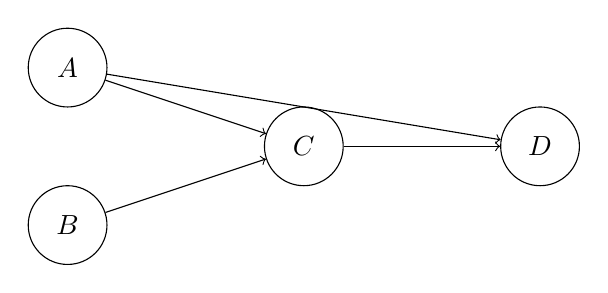
\begin{tikzpicture}
				\begin{scope}[xshift=8cm]
				\node[main node] (A) at (0,0) {$A$};
				\node[main node] (B) at (0,-2) {$B$};
				\node[main node] (C) at (3,-1) {$C$};
				\node[main node] (D) at (6,-1) {$D$};
				
				\draw[->] (A) to (C);
				\draw[->] (A) to (D);
				\draw[->] (B) to (C);
				\draw[->] (C) to (D);
				\end{scope}
			\end{tikzpicture}
			Figure~\ref{fig:glitchgraph} shows a dependency graph where \textit{C} observes changes from \textit{A} and \textit{B} and \textit{D} observes the resulting \textit{C} and also \textit{A}.
			When \textit{A} emits a change event, \textit{D} can not determine if \textit{C} has already consumed the change or not. 
			
			\item[Uniformity]
			
			\item[Abstraction]
			
			\item[Semantic distance]
		\end{description}

\section{Reactive programming}

	\subsection{Functional reactive programming (FRP)}

		first in functional languages by~\cite{Elliott}

		signals behaviour~\cite{Bainomugisha:2013}
	

\section{Scala.React}

	\subsection{First class events}

	\subsection{Reactor}

	\subsection{Embedded dataflow langugage}

\section{Evolution of reactive programming frameworks}

	with lambda-expressions and stream java added data-flow elements to the language for more declarative programming
	added in java 8 and already extended in java 9

	\subsection{Reactive databinding}

		Font-end frameworks inspired by the Flapjax reactive language~\cite{Meyerovich:2009}

		Metor example: ~\cite{hochhaus2016meteor}

		based on fl

	\subsection{Reactive streams}

\section{Conclusion}

%appendix: 
%javafx not glitch free stack overflow: https://stackoverflow.com/questions/25139257/terminology-what-is-a-glitch-in-functional-reactive-programming-rx

% Bibliography
\bibliographystyle{ACM-Reference-Format}
\bibliography{sources}

\end{document}
